% !TEX root = ../main.tex

\chapter{The SBN program at Fermilab and the ICARUS experiment}
\label{chap:icarus_detector}

\section{The Short Baseline Neutrino program at Fermilab}
%% BRIEF INTRODUCTION
The Short Baseline Neutrino experimental program at Fermi National Accelerator Laboratories aims to  draw a complete and consistent picture of the sterile neutrino scenario, depicted in detail in \autoref{chap:theory_introduction}. 
% The main physics goal of the SBN collaboration is to test with great sensitivity the presence of a fourth sterile neutrino state, as suggested by multiple experimental anomalies. 
To achieve a level of statistical significance greater than $5\sigma$ for the LSND-allowed region (at \SI{90}{\percent} CL), SBN will carry out precision searches, recording millions of NC and CC neutrino interactions on argon. 

The key to such high sensitivity, other than the great statistic of events collected, is the design paradigm of the program. It will employ the Liquid Argon Time Projection Chamber (LArTPC) technology \cite{rubbiaLiquidArgonTime1977}, with two functionally identical detectors placed at different distances from the neutrino source. This way, the oscillatory behaviour is observed by comparing the neutrino flux at the far detector with the ``control'' flux recorded at the near detector, reducing the systematic uncertainties related to neutrino production and neutrino interaction in argon. 

Albeit the original plan for a three-detector program \cite{acciarriProposalThreeDetector2015}, MicroBooNE finished its data-taking period in 2020, two years prior to ICARUS starting its data collection campaign and five prior to SBND, so the SBN program will perform a search for the sterile neutrino as a two-detector experiment \cite{acciarriProposalThreeDetector2015, machadoShortBaselineNeutrinoProgram2019}. 

Both collect data from the common Booster Neutrino Beam (BNB); additionally, the ICARUS detector is located such that it is sensible to off-axis neutrinos coming from the Neutrino at the Main Injector (NuMI) beam. 

ICARUS is the far detector for the SBN program, employing an active mass of \SI{476}{\tonne} of liquid argon (LAr), at a distance of \SI{600}{\meter} from the neutrino source; its position was chosen so as to maximise the oscillation probability. The ICARUS detector started its data taking independently from the SBN program in June of 2022, after the initial commissioning phase. It has now finished the fourth data collection campaign, collecting $\sim \SI{7.54e20}{POT}$ (proton-on-target), corresponding to about \num{e6} neutrino events.

At a distance of \SI{110}{\meter}, SBND is the near detector of the SBN program, with an active LAr mass of \SI{112}{\tonne}. After commissioning, it started data taking in December of 2024, joining the far detector and allowing for a precise knowledge of the neutrino flux. 

\paragraph{Oscillation measurements with a two-detector experiment} The main physics goal of the SBN program is the search for a fourth sterile neutrino state in the $3+1$ model. Using multiple LArTPC detectors, a high-sensitivity search for a high-$\Delta m^2$ splitting is possible by studying muon-neutrino oscillations in the $\PGnGm\to\PGnGm$ disappearance and $\PGnGm\to\PGne$ appearance channels. 

\begin{figure}
    \centering
    \includegraphics[width=\linewidth]{thesis/6_figures/SBN_sensitivity/appearance_signal.pdf}
    \caption[Electron neutrino appearance probability in the $3+1$ sterile oscillation scenario]{(a) and (b) show the oscillation probability for a \SI{700}{MeV} muon neutrino into an electron neutrino as a function of the length of the neutrino flight using two benchmark values of $(\sin^22\theta_{\PGm\Pe}, \Delta m^2)$. (c) and (d) show the same oscillation probability as a function of the neutrino energy. Additionally, the bottom panels show the far-over-near ratio. Adapted from \cite{machadoShortBaselineNeutrinoProgram2019}.}
    \label{fig:oscillation_2body_SBN}
\end{figure}

The oscillation probability for both channels is presented in \eqref{eq:2body_oscillation_sterile_disapp} and \eqref{eq:2body_oscillation_sterile_app} for the disappearance and appearance channels, respectively, with the assumption of the $3+1$ model. Looking at the $\PGnGm\to\PGne$ appearance channel, from the experimental results shown in \autoref{fig:all_experimental_searches}, the allowed parameter space lies in $\sin^22\theta_{\PGm\Pe} \in (\num{e-3},\num{e-1})$ and $\Delta m^2 \in (\num{e-1}, \num{e1})\ \si{eV^2}$; the location of the near and far detector  has been optimised to maximise the oscillation probability in this region of parameters. \autoref{fig:oscillation_2body_SBN} show $P(\PGnGm \rightarrow \PGne)$ for two benchmark values of $(\sin^22\theta_{\PGm\Pe}, \Delta m^2)$, assuming a neutrino energy of $\sim\SI{700}{MeV}$. Exploiting the strong correlations between the fluxes collected at the near and far detectors --- both use the same interaction medium and functionally identical revelation techniques --- the major impacting systematic uncertainties, which are those arising from the production mechanisms and the $\PGn$-Ar interaction cross-sections, can be mitigated in the two-detector configuration. 

With a planned collected statistics of \SI{6.6e20}{POT}, the $\PGnGm\to\PGnGm$ disappearance channel can also be probed to search for neutrino oscillation mediated by a sterile state. The unitarity of the $3+1$ PMNS matrix has to be preserved so that in the event of $\PGnGm\to\PGne$ appearance, meaning a nonzero value of $\sin^22\theta_{\PGm\Pe}$, a nonzero value of $\sin^22\theta_{\PGm\PGm}$, or a $\PGnGm\to\PGnGm$ disappearance signature, should be observed. 

Both channels will be studied to either pinpoint the correct $(\sin^22\theta, \Delta m^2)$ values or exclude some regions in the parameter space. \autoref{fig:sbn_2det} shows the projected excluded and allowed regions of the parameter space in both the \ref{sub@fig:nue_app_sbn_2det} $\PGne$-appearance and \ref{sub@fig:numu_disapp_sbn_2det} $\PGnGm$-disapperance channels of the two-detector operation of the SBN experiment. It should be noted that the projected \SI{6.6e20}{POT} was the original plan that was presented in the experiment proposal \cite{acciarriProposalThreeDetector2015}; however, BNB will operate until 2027, allowing the ICARUS detector to collect three times the statistics in standalone operation. 

\begin{figure}
    \centering
    \subfloat[]{\includegraphics[width=0.5\linewidth]{thesis/6_figures/SBN_sensitivity/nue_app_2det_newPOT_sensitivity_comparison.pdf}\label{fig:nue_app_sbn_2det}}
    \subfloat[]{\includegraphics[width=0.5\linewidth]{thesis/6_figures/SBN_sensitivity/numu_disapp_2det_newPOT_sensitivity_comparison.pdf}\label{fig:numu_disapp_sbn_2det}}
    \caption[SBN sensitivity plots in both appearance and disappearance channels]{\ref{sub@fig:nue_app_sbn_2det} and \ref{sub@fig:numu_disapp_sbn_2det} show, respectively, the expected sensitivity curves in the $\PGne$-appearance and $\PGnGm$-disappearance channels under the hypothesis of no observation (solid and dashed lines, respectively at $5\sigma$ and 99\% CL) and under the hypothesis of observing an oscillatory signature in both channels (filled regions). These projections account for a collected \SI{6.6e20}{POT} and a two-detector configuration. }
    \label{fig:sbn_2det}
\end{figure}

Additionally, since a nonzero value of both $\sin^2 2\theta_{\PGm\Pe}$ and $\sin^22\theta_{\PGm\PGm}$ leads to a nonzero value of $\sin^22\theta_{\Pe\Pe}$, both the ICARUS detector, making use of the Booster and NuMI neutrino beams, and the SBND detector, only with data from the Booster beam, will explore the $\PGne$-disappearance channel $\PGne\to\PGne$. The combined result of this multi-channel search will provide strong evidence in favour of or against the $3+1$ sterile neutrino scenario. 

\paragraph{Cross-sections and BSM physics} In addition to the primary physics goals, the SBN programme, with its two LArTPC detectors, delivers a rich physics opportunity. 

Starting from particle interaction in liquid argon, both SBND and ICARUS detectors will use the Booster and NuMI (ICARUS-only) neutrino beams to perform cross-section measurements, exploiting the great amount of collected data with both detectors. 
For SBND, the proximity with respect to the neutrino source leads to a very large flux collected by the detector --- each run approximately of \SI{2.2e20}{POT} corresponds to 1.5M $\PGnGm$ and \num{12000} $\PGne$s; 
the same measurements can be performed with the ICARUS detector, which at the moment benefits from a longer data collection period and an accumulated statistic of \SI{7.5e20}{POT} in standalone operation. The larger dimension of the ICARUS detector also allows for more contained events, where all the final state interactions (FSI) are contained inside the detector active volume, allowing for a better particle identification (PID). 
Additionally, the position of the ICARUS detector allows the collection of neutrinos from the NuMI beam at an off-axis angle of \SI{6}{\degree} with respect to BNB direction. 
The added value of the NuMI beam comes from the energy range it covers. 
Using protons from the Main Injector at an energy of \SI{120}{GeV}, it is able to cover the \qtyrange{1}{3}{GeV} energy range, which overlaps greatly with the DUNE operational energy range. Neutrinos from the NuMI beam will also feature an enriched electronic component from the three-body decay of the kaon, allowing for precise $\PGne$ cross-section measurements. At the moment of writing this thesis, two $\PGnGm$ charged current mesonless cross-section analyses, $\PGnGm\mathrm{CCN>1}\Pp0\PGp$ and $\PGnGm\mathrm{CCN}\Pp0\PGp$, are being carried on and are in the final phases before publication. 

Finally, exploiting the great tracking and calorimetric power of liquid argon TPCs, with exceptional precision and high-performance event reconstruction capabilities, opens up invaluable opportunities for new physics searches. Using high-intensity neutrino beams, with large statistics, it is possible to explore beyond standard model theories. A detailed description of possible searches is presented in refs. \cite{machadoShortBaselineNeutrinoProgram2019, acciarriProposalThreeDetector2015}. 
Recently the first physics paper by the ICARUS collaboration was published, exploring some of these BSM models involving the scalar sector using data from the NuMI beam \cite{icaruscollaborationSearchHiddenSector2025}. 

\subsection{Neutrino beam}

The location for the SBN programme was selected to make use of the already existing accelerator infrastructure at Fermilab. \autoref{fig:accelerator_complex} shows the FNAL accelerator complex schematic overview. This complex provides a powerful beam of neutrinos using protons extracted from the Booster accelerator, core to the operation of the SBN experiment, as well as multiple other particle beams (neutrinos and muons, as well as protons) which are employed in other experiments, such as the Neutrinos at the Main Injector Beam. 

The common starting point is the Linac (Linear accelerator), boosting protons up to \SI{400}{MeV} of energy (or $\sim\SI{954}{MeV}$ of momentum) using radiofrequency (RF) cavities. Accelerated protons are extracted and boosted to an energy of \SI{8}{GeV} within the Booster ring. 

\begin{figure}
    \centering
    \includegraphics[width=0.75\linewidth]{thesis/6_figures/detector/BNB_NuMI_beams.pdf}
    \caption[Fermilab Accelerator complex]{Schematics of the accelerator complex at Fermilab. Both Booster and NuMI neutrino beams serve the ICARUS detector, with different energy  ranges, \SI{700}{MeV} for BNB and \SI{2.5}{GeV} for NuMI. Taken from \cite{ainsworthHighIntensityOperation2020}.}
    \label{fig:accelerator_complex}
\end{figure}

From the Booster ring, a fraction of protons is extracted to be used for the Booster Neutrino Beam, whereas the remaining fraction is sent into the Main Injector accelerator. From there a second Neutrino beam is extracted, the Neutrinos at the Main Injector (NuMI) beam. 

\begin{figure}
    \centering
    \subfloat[]{\includegraphics[trim={0 6cm 0 6cm}, width=0.5\linewidth]{thesis/6_figures/beams/BNB_flux_lar1nd.pdf}\label{fig:BNB_flux_SBND}}
    \subfloat[]{\includegraphics[trim={0 6cm 0 6cm}, width=0.5\linewidth]{thesis/6_figures/beams/BNB_flux_icarus.pdf}\label{fig:BNB_flux_ICARUS}}

    \subfloat[]{\includegraphics[trim={0 0cm 0 0cm}, width=0.5\linewidth]{thesis/6_figures/beams/BNB_flux_ratio_icarus_lar1nd.pdf}\label{fig:BNB_flux_ICARUS_SBND_ratio}}
    \caption[BNB flux predictions at the near and far detectors]{Predictions of the neutrino flux as computed by the MicroBooNE collaboration \cite{aguilar-arevaloNeutrinoFluxPrediction2009} at distances of \SI{110}{m} \ref{sub@fig:BNB_flux_SBND} and \SI{600}{m} \ref{sub@fig:BNB_flux_ICARUS} from the beryllium target, i.e., for the SBND and ICARUS detectors, respectively. \ref{sub@fig:BNB_flux_ICARUS_SBND_ratio} shows the predicted ratio of the two fluxes under the hypothesis of no sterile-mediated oscillation anomaly. }
    \label{fig:BNB_flux}
\end{figure}

\paragraph{Booster Neutrino Beam} Protons accelerated up to \SI{8}{GeV} inside the Booster ring are extracted in groups of 81 bunches, each wide $\sim\SI{2}{ns}$ and \SI{19}{ns} apart. The repetition rate for the extraction, mainly limited by the focusing horn power supply, is of \SI{5}{\hertz}. Each pulse collides \SI{5e12}{p} onto a beryllium target. The target is embedded within a pulsed electromagnet (the ``horn'') that produces a toroidal magnetic field to focus positive secondary particles and defocus negative secondary particles emerging from proton-beryllium interactions. 

\paragraph{Neutrinos at the Main Injector off-axis beam}

\subsection{Liquid Argon Time Projection Chambers}

\subsection{The SBN near detector: SBND}

\section{The ICARUS-T600 detector}

\begin{sidewaysfigure}
    \centering
    \begin{tikzpicture}
        \node at (0,0) {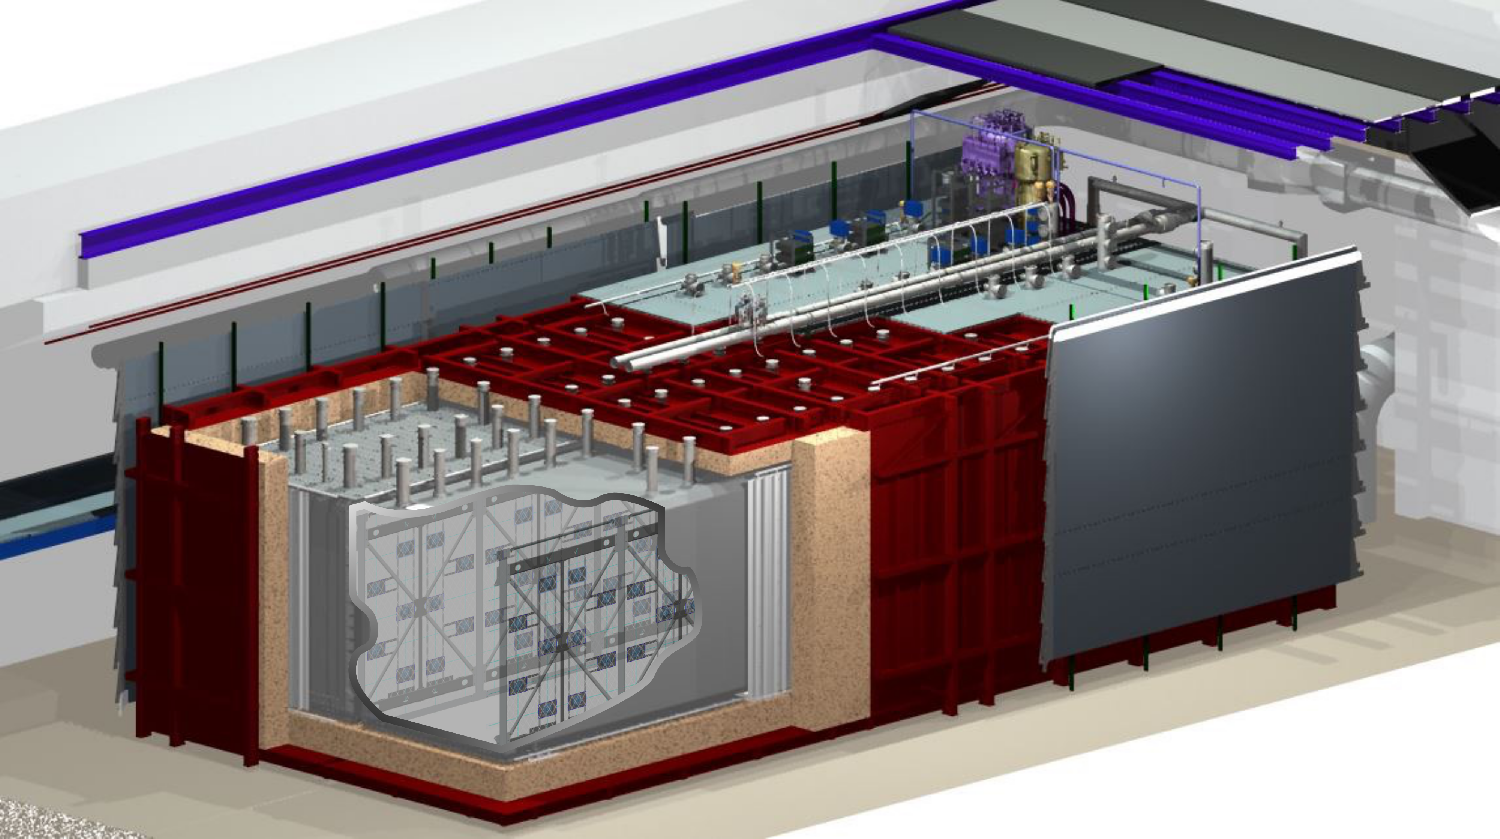
\includegraphics[width=\linewidth]{detector/SBN-FD_composite}};

        \draw[-*, white] (-1,2.5) node [left, white, fill=Gray!15!black] {TPC electronics} -- (0.5,2.25);
        \draw[-*, white] (-9,.5) node [right, white, fill=BrickRed] {Warm vessel} -- (-7.25,-1.5);
        \draw[-*, white] (4,2) node [right, white, fill=Plum!50!black] {Cryogenics} -- (3.25,3.5);
        \draw[-*, white] (7,-0.5) node [below, white, fill=Gray!15!black] {Top-CRT} -- (6.5,4);
        \draw[-*, white] (6,-1.75) node [right, white, fill=Gray!15!black] {Side-CRT} -- (5,-1);
        \draw[-*, white] (6,-3) node [above, white, fill=Gray!15!black] {Bottom-CRT} -- (3.5,-3.75);

        \draw[-*, white] (0,-4.5) node [below, white, fill=Gray!25!black] {East T300 cryostat} -- (-1,-3.5);
        \draw[-*, white] (-4.5,-4.5) node [left, white] {
            \begin{minipage}{4cm}
                \raggedleft
                TPC wireplanes + PMTs
            \end{minipage}} -- (-2.5,-2.5);

        \draw[-Latex, white] (-7,-3.5) -- (-7, -2.5) node[above] {$y$};
        \draw[-Latex, white] (-7,-3.5) -- (-6, -3.2) node[right] {$z$ (beam)};
        \draw[-Latex, white] (-7,-3.5) -- (-7.5, -3.35) node[left] {(drift) $x$};

        \draw[-*, black] (-4.5,5) node [left, black] {\SI{3}{m} concrete overburden} -- (-3,4.5);

        % \draw[step=1.0,white,thin] (-10,-5.5) grid (10,5.5);
        % \foreach \i in {-10,...,10} {
        %     \node [below] at (\i,-5.5) {$\i$};
        % }
        % \foreach \i in {-5,...,5} {
        %     \node [left] at (-10,\i) {$\i$};
        % }

        
    \end{tikzpicture}
    \caption[ICARUS detector illustration]{Illustration of the ICARUS T600 detector at Fermilab. Surrounding the warm vessel is the $4\pi$ coverage CRT. Above the warm vessel, the TPC readout warm electronics are placed, alongside the proximity cryogenics. Inside the warm vessel two identical (east and west) T300 modules are hosted, each containing two TPCs sharing a common cathode at the centre and two anode plane assemblies, one on each side.}
    \label{fig:ICARUS_scheme}
\end{sidewaysfigure}

\subsection{The ICARUS subsystems}

\paragraph{TPC}

\paragraph{Light collection system}

\paragraph{Cosmic ray tagger}


% Firstly proposed by Nobel laureate Carlo Rubbia \cite{Rubbia:1977zz}, the concept of Liquid Argon Time Projection Chambers (LArTPCs for short) was implemented in the Gran Sasso National Laboratories (LNGS) near L'Aquila (Italy) in the ICARUS (Imaging Cosmic And Rare Underground Signals) detector \cite{Bettini:1991fh, Cennini:1994pk, Cennini:1995tt, ICARUS:1995nrd}, which collected data between 2006 and 2011 \cite{Rubbia:2011ft}, alongside the OPERA, LVD and BOREXINO detectors from the CERN Neutrinos to Gran Sasso (CNGS) neutrino beam \cite{Kodama:2004db}. The main detectors for this project were the OPERA and ICARUS experiments, and were therefore called respectively CNGS1 and CNGS2.

% Today, the ICARUS T600 detector is one of the longest running LArTPC in existence. 

% After the results of the CNGS analysis were published the ICARUS detector moved in 2018 from LNGS, to the CERN facility, where it underwent a series of upgrades, both for electronics and in the liquid Argon purification system; serious upgrades were also performed on the exterior of the experiment where a cosmic ray tagger module was added; in 2020 the detector arrived to its current location in the SBN facility at Fermilab, where it has been detecting neutrinos since: mainly $\PGnGm$ and some $\PGne$s, from the Booster Neutrino Beam (BNB, on axis with the $z$ direction of the detector frame of reference) and from the Neutrino Main Injector (NuMI). 

% At the Short Baseline Neutrino (SBN) facility, the ICARUS experiment started its data run taking period in 2022 and has since ran thrice \cite{ICARUS:2023gpo}, with the latest data expected to be ready for the end of 2024 for the official analysis. Its younger brother, the SBND (Short Baseline Near Detector) experiment, finished the cryostat commissioning with some delays in 2023 and is now completing the commissioning of the cosmic ray tagger (CRT) modules, with the analysis on veto efficiency for the top CRT modules ongoing. 

% Joint efforts of the SBND and ICARUS detectors in the SBN collaboration will provide a highly efficient identification of neutrino interactions, strongly mitigating the possible sources of background and reducing the impact of systematics. 

% The combination of two nearly identical detectors allows for the measurement of neutrino oscillations over the distance in between the experiments, comparing the $\nu$s flux at \SI{110}{\meter} (SBND) and at \SI{600}{\meter} (ICARUS). 

% A third and a fourth experiment were also active in the BNB baseline, MiniBooNE (\mboone) and MicroBooNE (\uboone). The former completed its data taking period in 2018, and the latter was active between 2015 and 2021. Those two experiments provided strong ($\sim5\sigma$) evidence of event excess \cite{MiniBooNE:2018esg} in respect to what was expected (see figure \ref{fig:miniboone_results}). The main goal of the SBN collaboration is therefore to test this anomaly using data from BNB neutrinos. 

% In addition to this anomaly, ICARUS will also test the oscillation signal reported by the Neutrino-4 collaboration, hinting towards $\Delta m^2 \simeq \SI{7.26}{\electronvolt\squared}$ and $\sin^22\theta = 0.38$ ($3.5\sigma$ CL), both in $\PGne$ and $\PGnGm$ channels from BNB and NuMI.